The energy needs around the world has been increased a $60\%$ in the last 25 years and they are growing each day, mainly, due to the strong population growth (mundial population has increased in a $40\%$ between $1990$ and $2015$) and the fast development of emerging countries like China, India and Brazil. \cite{Renovables}. The prospects are that these energy necessities will keep increasing as it is shown in Figure \ref{fig:Wolrd_energy_consumption_a}, specially for countries which don't belong to the OECD like those mentioned earlier. In this figure one can see that the energy expected to be used in year 2040 is a factor two the energy used in year 2000.

Nowadays, as can be seen in Figure \ref{fig:Wolrd_energy_consumption_b}, the most used elements for energy production are liquid fuels, coal and natural gas, namely, natural elements. This fact has two problems. On the one hand, natural elements are limitated resources and this is a problem due to the huge increase of energy consumed worldwide and, on the other hand, obtaining energy from these natural elements produces large amounts of greenhouse gases (mainly $\ce{CO_2}$) which contribute to the environmental contamination, global warming, deforestation, etc. and this is a very big problem, specially right now, since United Nations (UN) did a communication on November 25, 2019 \cite{HighestCO2}, where they claimed that the lifestyle of the world population has not changed in the last years and, because of that, we achieved the highest level of the \ce{CO_2} in history.

\begin{figure}[]
 \centering
  \subfloat[]{
    \label{fig:Wolrd_energy_consumption_a}
    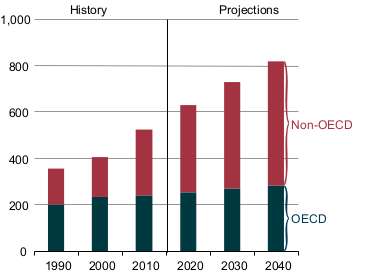
\includegraphics[width=0.5\textwidth]{2Introduction/world_energy_consumption_bar.png}}
  \subfloat[]{
    \label{fig:Wolrd_energy_consumption_b}
    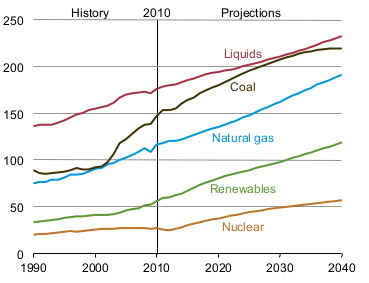
\includegraphics[width=0.5\textwidth]{2Introduction/world_energy_consumption_graph.png}}
 \caption{World energy consumption from 1990 up to the date and outlooks for the future until $2040$ (units in $10^{15}~Btu$) \cite{EIA}}
 \label{fig:Wolrd_energy_consumption} 
\end{figure}

In order to control these emissions, the United Nations in the Framework Convention about Climate Change (UNFCCC), has developed the Kyoto protocol \cite{Kyoto}. The objective of this protocol is to control and reduce the global negative environmental impact of greenhouse gases. It is focused on 6 different gases, carbon dioxide ($\ce{CO_2}$), methane ($\ce{CH_4}$), nitrous oxide ($\ce{N_2 O}$) and other three types of fluorinate industrial gases ($\ce{HFCs}$, $\ce{PFCs}$ and $\ce{SF6}$), which are related with the greenhouse effect and whose consecuence is the global warming. This convention only encourage to belonging countries to the United Nations to reduce their greenhouses gases emissions but this protocol commits the countries who has signed it to do so.

Therefore, we currently have a problem because, on the one hand, we want to maintain, even increase, this economic growth and for that we need to produce as much energy as we can but, on the other hand, we need to reduce the negative environmental impact. Hence, what we need is a energy source with which we can get a big quantity of energy with a very low greenhouse gases emissions. One possibility is the future nuclear fusion plants. They don't emit greenhouse gases and with its energy, which is practically limitless, we could satisfy the world's population needs of energy.

The largest representative in this sector is the ITER \cite{ITER} (International Thermonuclear Experimental Reactor) that is going to be the largest fusion reactor in the world. The ITER is currently under construction in Cadarache, France, and its objective is to provide the concept of sustained fusion. The nuclear reaction which ITER try to reproduce on earth is the one that uses deuterium ($\ce{^{2}_{1}H}$) and/or tritium ($\ce{^{3}_{1}H}$) because it is the only one whose requirements of temperature (several hundreds of millions degrees) and pressure can be achieved on earth. Among the possible combinations between both elements (Table \ref{tab:FusionReactions}), the choice of ITER is the nuclear reaction between deuterium and tritium in a 50:50 mixture because, as shown in Table \ref{tab:FusionReactions},  it is the nuclear reaction from which a maximum energy release is expected as shown in Table \ref{tab:FusionReactions}.

\begin{table}[htbp]
%%\centering
\begin{center}
\begin{tabular}{|c|c|c|}
\hline
Reaction & Products & Energy gain ($\MeV$) \\
\hline \hline \hline
$\ce{^{2}H}+\ce{^{3}H}$ & $\ce{^{4}He}+\ce{n}$ & $17.6$ \\ \hline
$\ce{^{3}H}+\ce{^{3}H}$ & $\ce{^{4}He}+2\ce{n}$ & $11.3$ \\ \hline
$\ce{^{2}H}+\ce{^{2}H}$ & $\ce{^{3}H}+\ce{^{1}H}$ & $3.98$ \\ \hline
$\ce{^{2}H}+\ce{^{2}H}$ & $\ce{^{3}He}+\ce{n}$ & $3.25$ \\ \hline
\end{tabular}
\caption{Fusion reactions between deuterium and tritium\cite{TritiumDocument}}
\label{tab:FusionReactions}
\end{center}
\end{table}

%%\vspace{-0.5cm}
Nevertheles, the fusion power plants are not yet commercially available as they are still in experimental development phase and its researchers need to solve some important problems like instabilitiy vortices, materials which withstand such high temperatures, etc. \cite{FusionCourse}. Hence, although we know that the nuclear fusion plants will be the energy of the future, nowadays, we have to wait until all their problems have been resolved.

Other energy source is the production of energy through the nuclear fusion reaction using Nuclear Power Plants (NPPs). With the NPPs we can practically avoid the problem of the greenhouse gas emission. We have to take into account that, although the nuclear fission reaction doesn't emit greenhouse gasses, the total procces to obtain the energy, which involves the uranium mining and milling, transport, uranium enrichment, etc., has a small contribution to the annual release of greenhouses gases. These emissions are difficult to estimate because, on the one hand, they depend on the NPP that we consider (for instance, there are studies which show that asian NPPs has higher emissions \cite{ComparationEmissions}) and, on the other hand, there are some tasks whose greenhouse gases emission are difficult to quantify\cite{ComparationEmissions}. 

There exist a study \cite{ComparationEmissions} which analyzes $19$ different studies of different NPPs. His estimation for the total greenhouses gases emision of a NPP is $66~\gram~\ce{CO_2} /\kilo\watt\hour$ which was obtained as a average of these $19$ studies considered. In Table \ref{tab:ComparationEmisions} this estimation is compared with the estimation for other energy kinds. In this table can be checked that the emissions due to NPPs is much more smaller, one order or more, than the emissions from burning natural elements.

\begin{table}[htbp]
%%\centering
\begin{center}
\begin{tabular}{|c|c|}
\hline
Technology & Estimate ($\gram~CO_2 /\kilo\watt\hour$)\\
\hline \hline
Wind & $9-10$ \\ \hline
Hydroelectric & $10-13$ \\ \hline
Biogas & $11$ \\ \hline
Solar thermal & $13$ \\ \hline
Biomass & $14-41$ \\ \hline
Solar PV & $32$ \\ \hline
Geothermal & $38$ \\ \hline
Nuclear & $66$ \\ \hline
Natural gas & $443$ \\ \hline
Fuel cell & $664$ \\ \hline
Diesel & $778$ \\ \hline
Heavy oil & $778$ \\ \hline
Coal & $960-1050$ \\ \hline
\end{tabular}
\caption{Estimations of $\ce{CO_2}$ emissions for several kinds of energy sources\cite{ComparationEmissions}}
\label{tab:ComparationEmisions}
\end{center}
\end{table}

NPPs are operational since more than 60 years and, nowadays, they are essential for providing a large part of the electic power that is used in the current world (more than 20\% in Spain as shown in Table \ref{tab:PercentageEnergySpain}). 

\begin{table}[htbp]
%%\centering
\begin{center}
\begin{tabular}{|c|c|c|c|}
\hline
Type of energy source & Contr. & Type of energy source & Contr.  \\
\hline \hline
Nuclear & $22.0\%$ & Wind & $20.9\%$  \\ \hline
Coal & $4.2\%$ & Hydraulics & $9.7\%$  \\ \hline
Combined Cycle & $20.1\%$ & Solar Photovoltaic & $3.5\%$  \\ \hline
Cogeneration & $11.8\%$ & Solar thermal & $2.0\%$  \\ \hline
No-renewable waste & $0.8\%$ & Other renewables & $1.4\%$  \\ \hline
Pumping turbine & $0.6\%$ & renewable waste & $0.3\%$  \\ \hline
 &  & \parbox{11em}{\centering Impoted balance of\\  international exchanges} & $2.7\%$\\ \hline
\end{tabular}
\caption{Contribution of each energy source to the total energy generated in Spain in 2019 \cite{PercentageEnergySpain}}
\label{tab:PercentageEnergySpain}
\end{center}
\end{table}

NPP is one of the cheapest source of energy production. It is a stable, as it doesn't depend on  meteorological parameters and, although there are other alternative energy sources which are being developed quickly  (photovoltaic, wind, tidal energy, etc.), even other concepts of energy production and saving (local production, solar roofs, energy efficiency, smart cities, etc.), today they are not developed enough to fully cover the population needs.  

The detractors of nuclear energy argue that NPPs facilitate nuclear proliferation or there are a risk of radiactive contamination and accidents like it happened in the past: Chernobyl, Fukushima and other accidents with lesser impact such as Three Mile Island, near to Pensilvania, USA \cite{ThreeMileIsland}.

Although we know that the nuclear energy is not the energy of the future since it produces nuclear waste which, by the moment, we don't know how we can eliminate, it is difficult that we leave to use nuclear energy because, now, we don't have a better solution for obtaining the energy which we need. 

In Spain the government is projecting to progressively close all NPP starting from year 2020, when the operative NPP reach the end of their useful life, by year 2030 \cite{CloseNPP}. 

In other countries like France, where $77\%$ of the energy consumed is obtained from nuclear sources, prefer to maintain their nuclear facilities and there even exist other countries that believe that nuclear energy is a safe investment like China which announced in 2016 that they were going to build 60 new nuclear reactors in the next dedade \cite{60ReactorsChina} or USA, who made an investment of 35 million of euros in 2019 for development and improvement of nuclear power plants \cite{35MillionsUSA}. 

In any case it is not important if we agree or not with nuclear energy source. The only important thing is that the nuclear energy production in the world is not going to stop in the next decade, in fact, it will increase as it is shown in Figure \ref{fig:Wolrd_energy_consumption_b}. Therefore the development of  different types of alarm systems is a good investment of both, time and money. Safety is not a negotiable aspect and there must be mechanisms that warn us of any malfunction of a nuclear power plant. Hence, our work has based on the development of a monitor that we can use as early alarm in case of any problem happen in a NPP.

Generally, a nuclear reactor, which is working in normal mode, is characterized by high stability and, therefore, by a constant emission of radioactive isotopes so the first alarm signs of any malfunctioning of a NPP is a variation of this radiactive emission rate.

Between all the radioactive elements which are produced in a nuclear power plant, the most frequently produced is tritium as the United States Department of Energy complex (U.S. DOE) \cite{FiberDetector1a} \cite{FiberDetector1b}  and other research facilities in China \cite{CommonEmissionTritium} have seen in their installations and in ground water, surface water, and process waste water around their facilities. However, as it will be shown in section \ref{sec:StateOfTheArt}, the current methods which is used for monitoring this radioactive element have some limitations. 

For these reasons, the radiactive element which we have chosen for monitoring with our early alarm system is tritium. We have focused our alarm system for working with NPPs but it could be also interesting for other tasks where tritium is involved like monitoring the behaviour of future fusion nuclear plants (ITER will need up to several tens of kilograms of tritium for working, which correspond to several $\tera\becquerel$ of tritium) or any nuclear research facility (tritium is a commun emission of these places \cite{FERMILAB},\cite{BrookHavenNationalLaboratory}),  tracking the movement of tritium contaminated plumes in ground water \cite{TrackingTritium} or demonstrate the compliance with the government agencies which fix the limit of the emitted radionuclides to the environmental. 

We have to take into account that the limit of the emission of each radioactive element depends on the government agency who manages it, and the regulation directives that is implemented in that place so, as a consequence, it is different in each country. For example, in Europe, these limits are fixed by the EURATOM Council Directive and the limit for tritium in drinking water, established in $2013$, is $A = 100~\becquerel/\liter$ \cite{100BqL}. In USA, these limits are set by the United States Environmental Protection Agency (U. S. EPA) and this limit for tritium in drinking water is $A = 20~\nano\curie/\liter = 740~\becquerel/\liter$ \cite{740BqL}, which was stablished in $2014$.

Tritium is normally produced in the water used in the nuclear reactor cooling system or the moderator of some NPPs. It is produced by neutron capture of the deuterium, which exist in the heavy water ($D_2 O$), semi-heavy water ($H D O$) or the deuterium which has been created by neutron capture in usual water ($H_2 O$). All these processes have a large probability to happen due to the huge neutron flux in the nuclear reactor, of the order of $10^{14} ~\ce{n} \, \cm^{-2} \second^{-1}$ \cite{CrossSeccionNeutrons}. 

The quantity of tritium will be different for each reactor type because, as we will see in the next section, the cross section of tritium production will depend on the materials which compose the reactor and its surroundings. Tritium emissions per year from different types of nuclear reactors can be seen in Table \ref{tab:TritiumEmisionsNPPs}. 

\begin{table}[htbp]
%%\centering
\begin{center}
\begin{tabular}{|c|c|c|}
\hline
Reactor type & Gaseous discharge ($\giga\becquerel/$y) & Liquid discharge ($\giga\becquerel/$y) \\
\hline \hline \hline
PWR & $3.70\cdot 10^{3}$ & $2.59\cdot 10^{4}$ \\ \hline
BWR & $1.85\cdot 10^{3}$ & $3.70\cdot 10^{3}$ \\ \hline
HWR & $7.40\cdot 10^{5}$ & $1.85\cdot 10^{5}$ \\ \hline
GCR & $7.40\cdot 10^{3}$ & $1.11\cdot 10^{4}$ \\ \hline
\end{tabular}
\caption{Emission of tritium per year from different types of nuclear reactors. The types of the nuclear reactor under consideration in this study are pressurized water reactor (PWR), boiled water reactor (BWR), Heavy water reactor (HWR) and Gas-Cooled Reactor (GCR) \cite{CommonEmissionTritium}}.
\label{tab:TritiumEmisionsNPPs}
\end{center}
\end{table} 

The tritium which is created in the water of the cooling system is finally released partially or totally in the environment. The most common way that tritium is released to the environment is $\ce{HTO}$ \cite{CommonEmissionTritium}.

Our alarm system will monitor the tritium activity in the river water in which the nuclear power plant releases the water used for its cooling system. It can also work for the water of the moderator in these types of NPP but it's not our objective because it's a close circuit so it's not a emission (unless the moderator is leaking, in which case our alarm system would detect it indirectly due to a variation of tritium activity in the water of the cooling system released to the environment).

The measurement of the tritium activity is one of the systematic environmental control which is performed during energy production by NPPs. It is normally done by liquid scintillation counter technic (LSC) which has a very good detection capability and precision but it has the inconvenient of providing a delayed results of about 1-2 days or even more. Liquid scintillation technique for the tritium measurement will be presented in section \ref{sec:StateOfTheArt}.

The detection of this tritium in quasi-real time ($<10~\min$) is important because of the following reasons:

\begin{enumerate}

\item{} It can warn us about the production of an excesive number of neutrons in the nuclear reactor due to the overheating of itself or a leakage of the water from the primary circuit of the cooling system in a nuclear power plant due to some break (perhaps because of an excesive preassure, other alarm sign of a malfunctioning of a nuclear reactor). Both causes could become in a very dangerous problems so the tritium detection in quasi-real time could be important in order to quickly detect and to solve it.

\item{} The water present in the secondary circuit of the cooling system, will be released to the evironment, usually rivers or seas, after using it for cooling purposes. Generally this water will be used later for human consumption, irrigation of all kind of plantations or it will arrive to places for fishing activities. 

Due to such a low legal limit in comparation with the activities of tritium inside of a nuclear reactor, it is possible that, if the nuclear power plant don't work correctly, the activity of tritium water released exceeds this limit and it will contaminate drinking water and plantations for more than 12 years (half-life of tiritium).

%%it become this water in no drinkable and these crops into inedibles. On top of that, the life time of tritium is more than 12 years so these places will remain contaminated during a lot of time. 

\item{} There exist a lot of rivers, which is used for cooling systems of the nuclear power plants, that are crossborders, that's, they are shared by several countries like our case as it will be seen in section \ref{sec:TritiumProject}. The emisión of an excessive tritium activity of one country could affect severely another country creating new international conflicts between them.

\end{enumerate}

Because of all these reasons it is very important that we have an alarm system which is capable of measuring such low tritium activities in quasi-real time. Nevertheless, as can be seen in section \ref{sec:StateOfTheArt}, at present, there are no commercially available detection system that could fulfill these requirements .

All these reasons have motivated the \textit{Tritium} project, whose objective is the development of a system for quasi-real time monitoring of low radioactive levels of tritium in water for security applications in nuclear power plants.